\section{Finite dimensional representations of \texorpdfstring{$\sll_2(k)$}{sl2(k)}}
Recall that the standard basis $(e,h,f)$ of $\sll_2(k)$ is given by
\[
 e = \begin{pmatrix} 0 & 1 \\ 0 & 0 \end{pmatrix}, \quad
 h = \begin{pmatrix} 1 & 0 \\ 0 & -1 \end{pmatrix}, \quad
 f = \begin{pmatrix} 0 & 0 \\ 1 & 0 \end{pmatrix}.
\]
This basis satisfies the relations
\[
 [h,e] = 2e, \quad
 [h,f] = -2f, \quad
 [e,f] = h.
\]


\begin{defi}
 Let $V$ be a representation of $\sll_2(k)$. For any $\lambda \in k$ let
 \[
  V_\lambda \coloneqq \{v \in V \mid h.v = \lambda v\}.
 \]
\end{defi}


\begin{lem}\label{lem: e and f moving the eigenspaces}
 Let $V$ a representation of $\g$ and $\lambda \in k$. Then
 \[
  e.V_\lambda \subseteq V_{\lambda+2}
  \quad\text{and}\quad
  f.V_\lambda \subseteq V_{\lambda-2}.
 \]
\end{lem}
\begin{proof}
 Let $v \in V_\lambda$. Then
 \begin{gather*}
  h.(e.v)
  = e.h.v + [h,e].v
  = \lambda e.v + 2e.v
  = (\lambda+2) e.v
 \shortintertext{and}
  h.(f.v)
  = h.f.v + [h,f].v
  = \lambda h.v - 2f.v
  = (\lambda-2) f.v.
 \qedhere
 \end{gather*}
\end{proof}


\begin{expl}
 Let $e_1$, $e_2$ be the standard basis of $V \coloneqq k^2$, which is the natural representation of $\sll_2(k)$. Then $h.e_1 = e_1$ and $h.e_2 = -1$, so $V_1 = k e_1$ and $V_{-1} = k e_2$ with $V = V_{-1} \oplus V_1$. Then $e.V_{-1} = V_1$ and $f.V_1 = V_{-1}$.
\end{expl}


\begin{thrm}
 \begin{enumerate}[leftmargin=*]
  \item
   For every $n \geq 1$ there exists a irreducible representation $V^{(n)}$ of $\sll_2(k)$ with $\dim_k V = n$.
  \item
   Let $V$ be an $n$-dimensional irreducible representation of $\sll_2(k)$ for some $n \geq 1$. Then
   \[
    V = V_{-n+1} \oplus V_{-n+3} \oplus \dotsb \oplus V_{n-3} \oplus V_{n-1}
   \]
   and $V_i$ is one-dimensional for every $i = -n+1, -n+3, \dotsc, n-3, n-1$. The action of $e$ on $V$ is given by
   \[
    e.V_i = V_{i+2} \quad \text{for every $i = -n+1, -n+3, \dotsc, n-3$}
   \]
   and the action of $f$ on $V$ by
   \[
    f.V_i = V_{i-2} \quad \text{for every $i = -n+3, \dotsc, n-3, n-1$}.
   \]
   More explicitely there exists a basis $v_1, \dotsc, v_n$ of $V$ with $v_i \in V_{-n-1+2i}$ for every $i = 1, \dotsc, n$, with respect to which respect the actions of $e$ and $f$ are given as in the following diagram, where the dashed arrows represent the action of $f$.
   \begin{center}
    \tikzsetnextfilename{irreducible_representation_of_sl2}
    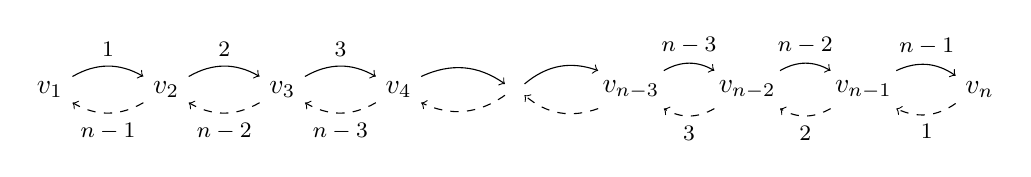
\begin{tikzpicture}[node distance = 4.2em]
     % the nodes
     \node (v1) {$v_1$};
     \node[right of = v1] (v2) {$v_2$};
     \node[right of = v2] (v3) {$v_3$};
     \node[right of = v3] (v4) {$v_4$};
     \node[right of = v4] (dots) {$\dotso$};
     \node[right of = dots] (vn-3) {$v_{n-3}$};
     \node[right of = vn-3] (vn-2) {$v_{n-2}$};
     \node[right of = vn-2] (vn-1) {$v_{n-1}$};
     \node[right of = vn-1] (vn) {$v_n$};
     % the action of e
     \draw[->, bend left] (v1) to node[above] {\footnotesize $1$} (v2);
     \draw[->, bend left] (v2) to node[above] {\footnotesize $2$} (v3);
     \draw[->, bend left] (v3) to node[above] {\footnotesize $3$} (v4);
     \draw[->, bend left] (v4) to (dots);
     \draw[->, bend left] (dots) to (vn-3);
     \draw[->, bend left] (vn-3) to node[above] {\footnotesize $n-3$} (vn-2);
     \draw[->, bend left] (vn-2) to node[above] {\footnotesize $n-2$} (vn-1);
     \draw[->, bend left] (vn-1) to node[above] {\footnotesize $n-1$} (vn);
     % the action of f
     \draw[->, bend left, dashed] (vn) to node[below] {\footnotesize $1$} (vn-1);
     \draw[->, bend left, dashed] (vn-1) to node[below] {\footnotesize $2$} (vn-2);
     \draw[->, bend left, dashed] (vn-2) to node[below] {\footnotesize $3$} (vn-3);
     \draw[->, bend left, dashed] (vn-3) to (dots);
     \draw[->, bend left, dashed] (dots) to (v4);
     \draw[->, bend left, dashed] (v4) to node[below] {\footnotesize $n-3$} (v3);
     \draw[->, bend left, dashed] (v3) to node[below] {\footnotesize $n-2$} (v2);
     \draw[->, bend left, dashed] (v2) to node[below] {\footnotesize $n-1$} (v1);
    \end{tikzpicture}
   \end{center}
   In particular $V$ is up to isomorphism the unique $n$-dimensional irreducible representation of $\sll_2(k)$.
 \end{enumerate}
\end{thrm}
\begin{proof}
 \begin{enumerate}[leftmargin=*]
  \item
   Let $\sll_2(k)$ act on $V \coloneqq k[x,y]$ via
   \[
    \sll_2(k) \to \gl(V), \quad
    e \mapsto y\dd{x}, \quad
    h \mapsto y\dd{y}-x\dd{x}, \quad
    f \mapsto x\dd{y}.
   \]
   It was already shown in Examples~\ref{expls: representations of Lie algebras} that this defines a representation of $\sll_2(k)$. Let $V^{(n)} \subseteq V$ be the linear subspace consisting of the homogeneous polynomials of degree $n-1$, i.e.\
   \[
    V^{(n)} = \vspan_k\left( x^{n-1}, x^{n-2} y, \dotsc, x y^{n-2}, y^{n-1} \right).
   \]
   Then $V^{(n)}$ is an $n$-dimensional subrepresentation of $V$.
   
   Let $U \subseteq V^{(n)}$ be a nonzero subrepresentation. If $p \in U$ is a nonzero polynomial then by applying $f$ often enough it follows that $x^{n-1} \in U$, from which it follows from applying $e$ often enough that $x^{n-i} y^{i-1} \in U$ for every $i = 1, \dotsc, n$. Hence $U = V$. So $V^{(n)}$ is an irreducible representation of $\sll_2(k)$.
   
  \item
   Because $V \neq 0$ is finite dimensional and $k$ is algebraically closed there exists some $\lambda \in k$ with $V_\lambda \neq 0$. Because $v$ is finite dimensional $\lambda$ can be choosen such that $V_{\lambda-2} = 0$. Let $w \in V_\lambda$ with $w \neq 0$. Set
   \[
    w_i \coloneqq e^i.w \quad \text{for every $i \in \N$}.
   \]
   \begin{claim*}
    \begin{enumerate}[leftmargin=*]
     \item
      $h.w_i = (\lambda+2i) w_i$ for every $i \in \N$.
     \item
      $f.w_0 = 0$ and $f.w_{i+1} = -(i+1)(\lambda+i)w_i$ for every $n \in \N$.
    \end{enumerate}
   \end{claim*}
   \begin{proof}
    \begin{enumerate}[leftmargin=*]
     \item
      This follows from $w \in V_\lambda$ and Lemma~\ref{lem: e and f moving the eigenspaces}.
     \item
      From $w_0 = w \in V_\lambda$ and Lemma~\ref{lem: e and f moving the eigenspaces} it follows that $f.w_0 \in V_{\lambda-2}$. Because $V_{\lambda-2} \neq 0$ it follows that $f.w_0 = 0$.
      
      The second formula will be shown by induction over $i \in \N$. It holds for $i = 0$ because
      \[
       f.w_1
       = f.e.w_0
       = [f,e].w_0 - e.f.w_0
       = -h.w_0
       = -\lambda w_0.
      \]
      Now let $i > 0$ and suppose the formula holds for $i-1$. Then
      \begin{align*}
       f.w_{i+1}
       &= f.e.w_i
       = [f,e].w_i + e.f.w_i
       = -h.w_i + e.f.w_i \\
       &= -(\lambda+2i) w_i -i(\lambda+i-1) e.w_{i-1} \\
       &= (-\lambda -2i -i\lambda -i^2 +i) w_i
       =  -(i+1)(\lambda+i) w_i.
      \qedhere
      \end{align*}

     \qedhere
    \end{enumerate}
   \end{proof}
   
   Because $w_i \in V_{\lambda+2i}$ for every $i \in \N$ with $w_0 = v \neq 0$ and $V$ is finite dimensional it follows that there exists a maximal $m \in \N$ such that $w_0, \dotsc, w_m$ are nonzero but $w^{m+1} = 0$. By the previous claim $\vspan_k(w_0, \dotsc, w_m)$ is a subrepresentation of $V$. Because $V$ is irreducible it follows that $V = \vspan_k(w_0, \dotsc, w_m)$. Because $w_0, \dotsc, w_m$ are linearly independent it follows that $w_0, \dotsc, w_m$ is a basis of $V$.
   
   As $V$ is $n$-dimensional it follows that $m = n-1$. By the claim
   \[
    0
    = f.w_n
    = f.w_{(n-1)+1}
    = -n(\lambda+n-1).w_{n-1}
   \]
   and therefore $\lambda = -n+1$. Because $w_i \in V_{\lambda + 2i} = V_{-n+1+2i}$ for every $i \in \N$ it follows that
   \[
    V
    = kw_0 \oplus \dotsb \oplus kw_{n-1}
    = V_{-n+1} \oplus V_{-n+3} \oplus \dotsb \oplus V_{n-3} \oplus V_{n-1}
   \]
   with $V_i$ being one-dimensional for every $i = -n+1, -n+3, \dotsc, n-3, n-1$. From the definition of $w_0, \dotsc, w_{n-1}$ and the claim it follows that the actions of $e$ and $f$ are given as in the following diagram, where the dashed arrows represent the action of $f$.
   \begin{center}
    \tikzsetnextfilename{irreducible_representation_of_sl2_construction}
    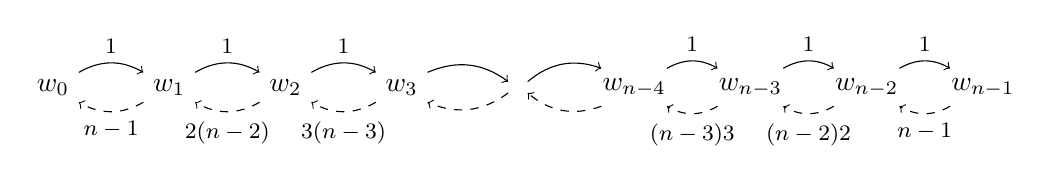
\begin{tikzpicture}[node distance = 4.2em]
     % the nodes
     \node (w0) {$w_0$};
     \node[right of = w0] (w1) {$w_1$};
     \node[right of = w1] (w2) {$w_2$};
     \node[right of = w2] (w3) {$w_3$};
     \node[right of = w3] (dots) {$\dotso$};
     \node[right of = dots] (wn-4) {$w_{n-4}$};
     \node[right of = wn-4] (wn-3) {$w_{n-3}$};
     \node[right of = wn-3] (wn-2) {$w_{n-2}$};
     \node[right of = wn-2] (wn-1) {$w_{n-1}$};
     % the action of e
     \draw[->, bend left] (w0) to node[above] {\footnotesize $1$} (w1);
     \draw[->, bend left] (w1) to node[above] {\footnotesize $1$} (w2);
     \draw[->, bend left] (w2) to node[above] {\footnotesize $1$} (w3);
     \draw[->, bend left] (w3) to (dots);
     \draw[->, bend left] (dots) to (wn-4);
     \draw[->, bend left] (wn-4) to node[above] {\footnotesize $1$} (wn-3);
     \draw[->, bend left] (wn-3) to node[above] {\footnotesize $1$} (wn-2);
     \draw[->, bend left] (wn-2) to node[above] {\footnotesize $1$} (wn-1);
     % the action of f
     \draw[->, bend left, dashed] (wn-1) to node[below] {\footnotesize $n-1$} (wn-2);
     \draw[->, bend left, dashed] (wn-2) to node[below] {\footnotesize $(n-2)2$} (wn-3);
     \draw[->, bend left, dashed] (wn-3) to node[below] {\footnotesize $(n-3)3$} (wn-4);
     \draw[->, bend left, dashed] (wn-4) to (dots);
     \draw[->, bend left, dashed] (dots) to (w3);
     \draw[->, bend left, dashed] (w3) to node[below] {\footnotesize $3(n-3)$} (w2);
     \draw[->, bend left, dashed] (w2) to node[below] {\footnotesize $2(n-2)$} (w1);
     \draw[->, bend left, dashed] (w1) to node[below] {\footnotesize $n-1$} (w0);
    \end{tikzpicture}
   \end{center}
   The desired basis $v_1, \dotsc, v_n$ can now be defined as
   \[
    v_i \coloneqq \frac{w_{i-1}}{(i-1)!}
    \quad \text{for every $i = 1, \dotsc, n$}.
   \]
  \qedhere
 \end{enumerate}
\end{proof}

















